\section{Casi d'uso}

\subsection{Attori dei casi d'uso}

\subsubsection{Attori primari}
\begin{figure}[H]
		\centering
		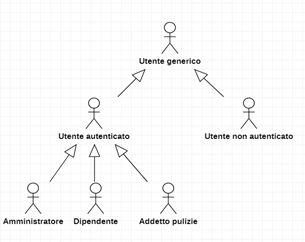
\includegraphics[width=10cm]{res/images/utentigenerali.png}
		\caption{Gerarchia degli attori principali}
		\label{fig:Gerarchia attori principali}
	\end{figure}

\textbf{Utente generico}\\
Si riferisce ad un utente generico che accede alla piattaforma.\\
\\
\textbf{Utente non autenticato}\\
Si riferisce ad un utente generico che non ha ancora effettuato l’autenticazione alla piattaforma.\\
\\
\textbf{Utente autenticato}\\
Si riferisce ad un utente generico che si è autenticato nel sistema con la procedura di login.\\
\\
\textbf{Amministartore}\\
Si riferisce ad un utente che si è autenticato nel sistema con il ruolo di amministratore.\\
\\
\textbf{Dipendente}\\
Si riferisce ad un utente che si è autenticato nel sistema con il ruolo di dipendente.\\
\\
\textbf{Addetto pulizie}\\
Si riferisce ad un utente che si è autenticato nel sistema con il ruolo di addetto alle pulizie.\\

\subsubsection{Attori secondari}

\subsection{Elenco dei casi d'uso}
